\chapter{Proverb 1}

\begin{figure}
  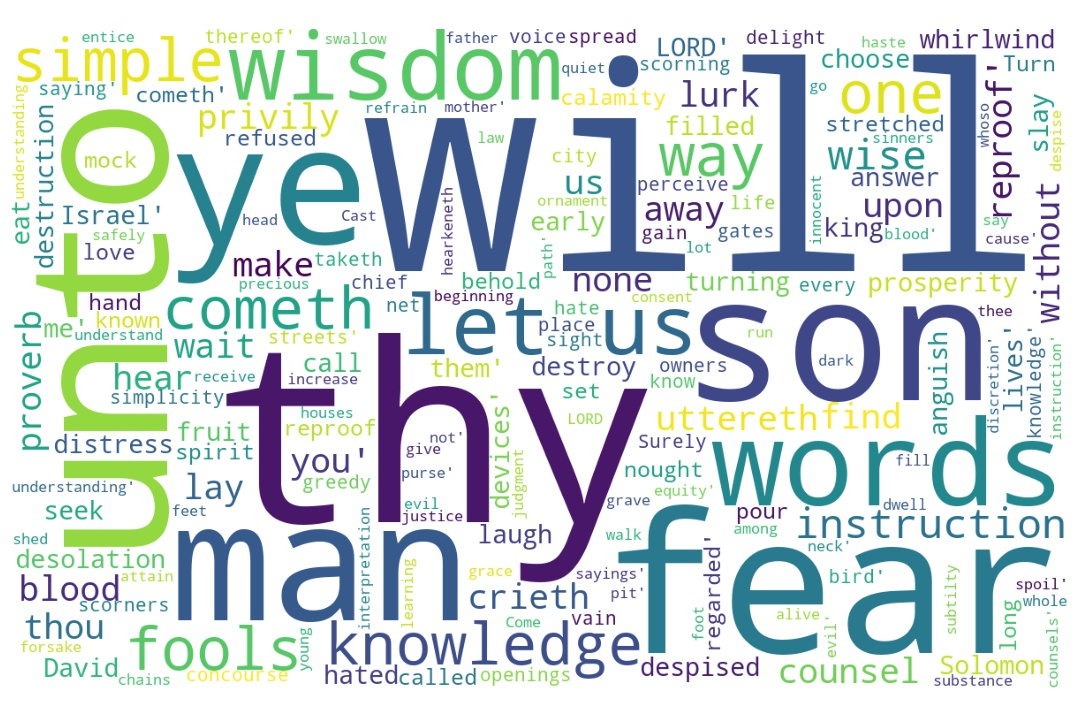
\includegraphics[width=\linewidth]{20OT-Proverbs/Proverb1-WordCloud.jpg}
  \caption{Proverb 1 Word Cloud}
  \label{fig:Proverb 1 word Cloud}
\end{figure}

\marginpar{\scriptsize \centering \fcolorbox{bone}{lime}{\textbf{PURPOSES FOR PROVERBS}}\\ (Proverb 1:1--6) 
\begin{compactenum}[I.][8]
	\item To \textbf{Know}  \index[scripture]{Proverbs!Pro 01:02}(Pro 1:2)
	\begin{compactenum}[A.]
		\item Wisdom
		\item Instruction
	\end{compactenum}
	\item To \textbf{Perceive}  \index[scripture]{Proverbs!Pro 01:02}(Pro 1:2)
	\begin{compactenum}[A.]
		\item Words of Understanding
	\end{compactenum}
	\item To \textbf{Receive}  \index[scripture]{Proverbs!Pro 01:03}(Pro 1:3)
	\begin{compactenum}[A.]
		\item Instruction of wisdom
		\item Instruction of justice
		\item Instruction of judgment
		\item Instruction of equity
	\end{compactenum}
	\item To \textbf{Give}  \index[scripture]{Proverbs!Pro 01:04}(Pro 1:4)
	\begin{compactenum}[A.]
		\item Subtilty to the simple
		\item Knowkledge and discretion to a young man
	\end{compactenum}
	\item To \textbf{Understand}  \index[scripture]{Proverbs!Pro 01:06}(Pro 1:6)
	\begin{compactenum}[A.]
		\item A proverb
		\item The interpreataion
		\item Words of the oise
		\item Dark sayings
	\end{compactenum}
\end{compactenum} }

\marginpar{\scriptsize \centering \fcolorbox{bone}{yellow}{\textbf{THE CALL OF WISDOM}}\\ (Proverb 1:20--33) 
\begin{compactenum}[I.][8]
\item An \textbf{Obvious Recruitment}  \index[scripture]{Proverbs!Pro 01:21}(Pro 1:21)
\item \textbf{Oblivious Rebels} \index[scripture]{Proverbs!Pro 01:22}(Pro 1:22)
\item An \textbf{Obstinant Response} \index[scripture]{Proverbs!Pro 01:22}(Pro 1:22)
\item The \textbf{Obstacle of Rejection} \index[scripture]{Proverbs!Pro 01:22}(Pro 1:22)
\item \textbf{Obedience Required} \index[scripture]{Proverbs!Pro 01:22}(Pro 1:22)
\item \textbf{Obeisance in Response} \index[scripture]{Proverbs!Pro 01:22}(Pro 1:22)
\item An \textbf{Outstanding Result} \index[scripture]{Proverbs!Pro 01:33}(Pro 1:33)
\end{compactenum} }

\marginpar{\scriptsize \centering \fcolorbox{black}{black}{\textbf{\textcolor[cmyk]{0,0,0,0}{DOCTRINE OF SELF-CONTROL}}}\\ (Proverb 1:4) 
\begin{compactenum}[I.][8]
\item The \textbf{Consideration}  \index[scripture]{Proverbs!Pro 01:04}(Pro 1:4)
\item The \textbf{Counsel}  \index[scripture]{Proverbs!Pro 01:06}\index[scripture]{Proverbs!Pro 01:25}\index[scripture]{Proverbs!Pro 01:30}(Pro 1:6, 25, 30)
\item The \textbf{Calamity}  \index[scripture]{Proverbs!Pro 01:26}\index[scripture]{Proverbs!Pro 01:32}(Pro 1:26, 32)
\item The \textbf{Chains}  \index[scripture]{Proverbs!Pro 01:09}(Pro 1:9)
\item The \textbf{Consent}  \index[scripture]{Proverbs!Pro 01:10}(Pro 1:10)
\item The \textbf{Choices}  \index[scripture]{Proverbs!Pro 01:15}(Pro 1:15)
\item The \textbf{Call}  \index[scripture]{Proverbs!Pro 01:24}(Prov 1:24) of wisdom
\end{compactenum} }

\marginpar{\scriptsize \centering \fcolorbox{bone}{blue}{\textbf{\textcolor{white}{THE CALL OF THE WILD}}}\\ (Proverb 1:10-19) 
\begin{compactenum}[I.][8]
\item Their \textbf{Way}  \index[scripture]{Proverbs!Pro 01:11}\index[scripture]{Proverbs!Pro 01:15-16}(Pro 1:11,15-16)
\item The \textbf{Waiting}  \index[scripture]{Proverbs!Pro 01:11}\index[scripture]{Proverbs!Pro 01:18}(Pro 1:11, 18)
\item Their \textbf{Wantonness}  \index[scripture]{Proverbs!Pro 01:13}(Pro 1:13)
\item The \textbf{Warnings}  \index[scripture]{Proverbs!Pro 01:10}\index[scripture]{Proverbs!Pro 01:15}(Pro 1:10, 15)
\end{compactenum} }

\marginpar{\scriptsize \centering \fcolorbox{bone}{orange}{\textbf{MARKS OF A FOOL}}\\ (Proverb 1:7) 
 \begin{compactenum}[I.][8]
	\item \textbf{Despises wisdom} \index[scripture]{Proverbs!Pro 01:07}(Pro 1:7).
	\item \textbf{Makes a mock at Sin} \index[scripture]{Proverbs!Pro 14:09}(Pro 14:9).
	\item \textbf{Meddles in other people’s business} \index[scripture]{Proverbs!Pro 20:03}(Pro 20:3).
	\item \textbf{Slanders people} \index[scripture]{Proverbs!Pro 10:18}(Pro 10: 18).
	\item \textbf{Imitates a dog eating vomit} \index[scripture]{Proverbs!Pro 26:11}(Pro 26: 11).
	\item \textbf{Has his eyes in the ends of the earth} \index[scripture]{Proverbs!Pro 17:24}(Pro 17:24).
	\item \textbf{Resists punishment for correction} \index[scripture]{Proverbs!Pro 17:10}(Pro 17: 10).
	\item \textbf{Trusts in his own heart} \index[scripture]{Proverbs!Pro 28:26}(Pro 28:26)
\end{compactenum} }

\footnote{\textcolor[cmyk]{0.99998,1,0,0}{\hyperlink{TOC}{Return to end of Table of Contents.}}}\footnote{\href{https://www.audioverse.org/english/audiobibles/books/ENGKJV/O/Prov/1}{\textcolor[cmyk]{0.99998,1,0,0}{Proverbs Audio}}}\textcolor[cmyk]{0.99998,1,0,0}{The proverbs of Solomon the son of David, king of Israel;}
[2] \textcolor[cmyk]{0.99998,1,0,0}{To\textcolor{jungle}{$_{12}$}  \fcolorbox{bone}{lime}{know} wisdom and instruction; to  \fcolorbox{bone}{lime}{perceive} the words of \fcolorbox{bone}{MYGOLD}{understanding};}
[3] \textcolor[cmyk]{0.99998,1,0,0}{To\textcolor{jungle}{$_{23}$}  \fcolorbox{bone}{lime}{receive} the instruction of wisdom, justice, and judgment, and equity;}
[4] \textcolor[cmyk]{0.99998,1,0,0}{To\textcolor{jungle}{$_{34}$}  \fcolorbox{bone}{lime}{give} subtilty to the simple, to the young man knowledge and discretion.}
[5] \textcolor[cmyk]{0.99998,1,0,0}{A\textcolor{jungle}{$_{47}$} wise \emph{man} will hear, and will increase learning; and a man of \fcolorbox{bone}{MYGOLD}{understanding} shall attain unto wise counsels:}
[6] \textcolor[cmyk]{0.99998,1,0,0}{To\textcolor{jungle}{$_{66}$}  \fcolorbox{bone}{lime}{understand} a proverb, and the interpretation; the words of the wise, and their dark sayings.}\\
\\
\P \textcolor[cmyk]{0.99998,1,0,0}{The\textcolor{jungle}{$_{82}$} fear of the LORD \emph{is} the beginning of knowledge: \emph{but} fools despise wisdom and instruction.}
[8] \textcolor[cmyk]{0.99998,1,0,0}{My\textcolor{jungle}{$_{98}$} son, hear the instruction of thy father, and forsake not the law of thy mother:}
[9] \textcolor[cmyk]{0.99998,1,0,0}{For\textcolor{jungle}{$_{114}$} they \emph{shall} \emph{be} an ornament of grace unto thy head, and chains about thy neck.}\\
\\
\P \textcolor[cmyk]{0.99998,1,0,0}{My\textcolor{jungle}{$_{130}$} son, if sinners entice thee, consent thou not.}
[11] \textcolor[cmyk]{0.99998,1,0,0}{If\textcolor{jungle}{$_{139}$} they say, Come with us, let us lay wait for blood, let us lurk privily for the innocent without cause:}
[12] \textcolor[cmyk]{0.99998,1,0,0}{Let\textcolor{jungle}{$_{160}$} us swallow them up alive as the grave; and whole, as those that go down into the pit:}
[13] \textcolor[cmyk]{0.99998,1,0,0}{We\textcolor{jungle}{$_{179}$} shall find all precious substance, we shall fill our houses with spoil:}
[14] \textcolor[cmyk]{0.99998,1,0,0}{Cast\textcolor{jungle}{$_{192}$} in thy lot among us; let us all have one purse:}
[15] \textcolor[cmyk]{0.99998,1,0,0}{My\textcolor{jungle}{$_{204}$} son, walk not thou in the way with them; refrain thy foot from their path:}
[16] \textcolor[cmyk]{0.99998,1,0,0}{For\textcolor{jungle}{$_{220}$} their feet run to evil, and make haste to shed blood.}
[17] \textcolor[cmyk]{0.99998,1,0,0}{Surely\textcolor{jungle}{$_{232}$} in vain the net is spread in the sight of any bird.}
[18] \textcolor[cmyk]{0.99998,1,0,0}{And\textcolor{jungle}{$_{245}$} they lay wait for their \emph{own} blood; they lurk privily for their \emph{own} lives.}
[19] \textcolor[cmyk]{0.99998,1,0,0}{So\textcolor{jungle}{$_{260}$} \emph{are} the ways of every one that is greedy of gain; \emph{which} taketh away the life of the owners thereof.}\\
\\
\P \textcolor[cmyk]{0.99998,1,0,0}{Wisdom\textcolor{jungle}{$_{281}$} crieth without; she uttereth her voice in the streets:}
[21] \textcolor[cmyk]{0.99998,1,0,0}{\fcolorbox{bone}{yellow}{She\textcolor{jungle}{$_{291}$} crieth} in the chief place of concourse, in the openings of the gates: in the city she uttereth her words, \emph{saying},}
[22] \textcolor[cmyk]{0.99998,1,0,0}{How\textcolor{jungle}{$_{313}$} long, ye simple ones, will ye love simplicity? and the \fcolorbox{bone}{yellow}{scorners} delight in their \fcolorbox{bone}{yellow}{scorning}, and fools \fcolorbox{bone}{yellow}{hate knowledge?}}
[23] \textcolor[cmyk]{0.99998,1,0,0}{Turn\textcolor{jungle}{$_{333}$} you at my reproof: behold, I will pour out my spirit unto you, I will make known my words unto you.}\\
\\
\P \textcolor[cmyk]{0.99998,1,0,0}{Because\textcolor{jungle}{$_{355}$} I have called, and ye refused; I have stretched out my hand, and no man regarded;}
[25] \textcolor[cmyk]{0.99998,1,0,0}{But\textcolor{jungle}{$_{372}$} ye have set at nought all my counsel, and would none of my reproof:}
[26] \textcolor[cmyk]{0.99998,1,0,0}{I\textcolor{jungle}{$_{387}$} also will laugh at your calamity; I will mock when your fear cometh;}
[27] \textcolor[cmyk]{0.99998,1,0,0}{When\textcolor{jungle}{$_{401}$} your fear cometh as desolation, and your destruction cometh as a whirlwind; when distress and anguish cometh upon you.}
[28] \textcolor[cmyk]{0.99998,1,0,0}{Then\textcolor{jungle}{$_{421}$} shall they call upon me, but I will not answer; they shall seek me early, but they shall not find me:}
[29] \textcolor[cmyk]{0.99998,1,0,0}{For\textcolor{jungle}{$_{443}$} that they hated knowledge, and did not choose the fear of the LORD:}
[30] \textcolor[cmyk]{0.99998,1,0,0}{They\textcolor{jungle}{$_{457}$} would none of my counsel: they despised all my reproof.}
[31] \textcolor[cmyk]{0.99998,1,0,0}{Therefore\textcolor{jungle}{$_{468}$} shall they eat of the fruit of their own way, and be filled with their own devices.}
[32] \textcolor[cmyk]{0.99998,1,0,0}{For\textcolor{jungle}{$_{486}$} the turning away of the simple shall slay them, and the prosperity of fools shall destroy them.}
[33] \textcolor[cmyk]{0.99998,1,0,0}{But\textcolor{jungle}{$_{504}$} whoso hearkeneth unto me \fcolorbox{bone}{yellow}{shall dwell safely}, and shall be quiet from fear of evil\textcolor{jungle}{$_{519}$}.}



